%--------------------------------------------------
%	Chapter 5. GNN Pattern Recognition Algorithm
%--------------------------------------------------

\chapter{Graph Neural Network Pattern Recognition Algorithm}\label{chapter-5}

Once compatible hit-pairs have been established, they can be used to build a graph network to represent a particle collision event. This chapter presents a novel pattern recognition algorithm utilising GNN architectures to prune connections in such a network, in order to reconstruct tracks in a silicon based Pixel detector. The application is focused on the Pixel detector, with the aim that the approach will serve as a sophisticated track seeding technique for Pixel hits and form preliminary track candidates. These seeds can be extended into the Strips using standard track following. Such an approach could be efficient for saving computational resources if the GNN does not produce large proportions of fake tracks. The ultimate aim of this work is to develop a realistic algorithm for fast track reconstruction that can be deployed in future high-luminosity phases of particle detector experiments. This research was presented at the 2022 Connecting the Dots (CTD) conference at the University of Princeton USA and is currently under review for publication in the Springer Journal: Computing for Software and Big Science \cite{Lad_2023_gnn}. Sections \ref{gnn-algorithm-overview} to \ref{gnn-kf-implementation} present an overview and detailed breakdown of each stage of the algorithm and Section \ref{gnn-application-toy-model} illustrates a simple application on a toy model.



\section{Algorithm Overview}
\label{gnn-algorithm-overview}
The GNN based pattern recognition algorithm is considered as an iterative mixture reduction task, that allows deactivating incompatible connections (GNN edges termed as outliers) in order to improve track parameter estimates and iteratively extract track candidates. 

Individual hits or clusters of hits are modelled as graph nodes and track segments are modelled as graph edges. Once the graph network is constructed, each edge is modelled as a Gaussian state in order to approximate the local track state probability density. Therefore, each node is initialised with a Gaussian mixture of track states, local to its neighbourhood of connections.

After initialisation, the network evolves iteratively, where an iteration is made up of three main stages illustrated in Figure \ref{fig:flowchart}. The first stage comprises of Gaussian Mixture Reduction (GMR). This involves a traditional ML approach, whereby compatible Gaussian states are grouped together using clustering techniques and outlier states can be identified. This stage is followed by information aggregation by leveraging message passing between nodes in a given neighbourhood. The compatibility of neighbouring states can be assessed via extrapolation, in order to improve local track parameters using neighbourhood information. The third stage involves updating the network state at each node, as certain connections are deactivated. After stages one and two a graph splitting algorithm is applied to identify good track candidates, and if discovered they are extracted. 

Unlike traditional methodologies whereby Multi-Layered Perceptrons (MLPs) are employed for deep learning strategies, the proposed GNN leverages simplified KFs embedded in the network and are used for two main purposes. Firstly, the KF is used as a mechanism for information propagation, in order to iteratively improve the precision of track parameters. Secondly, the KF is used in extraction of track candidates compatible with particle motion model. This allows the model to efficiently exploit a prior knowledge about charged particle dynamics as the network evolves.

The excitation and inhibition rules of individual edge connections are designed to facilitate the “simple-to-complex” approach for “hits-to-tracks” association, such that the network starts with low hit density regions of an event and gradually progresses towards more complex areas. As the network evolves, the uncertainty in local track orientation decreases until there are no more track candidates that fulfil the criteria for a good track. This is the end state of the network where isolated nodes, track fragments and unresolved ambiguities will remain.

\begin{figure}[htbp]
    \centering
    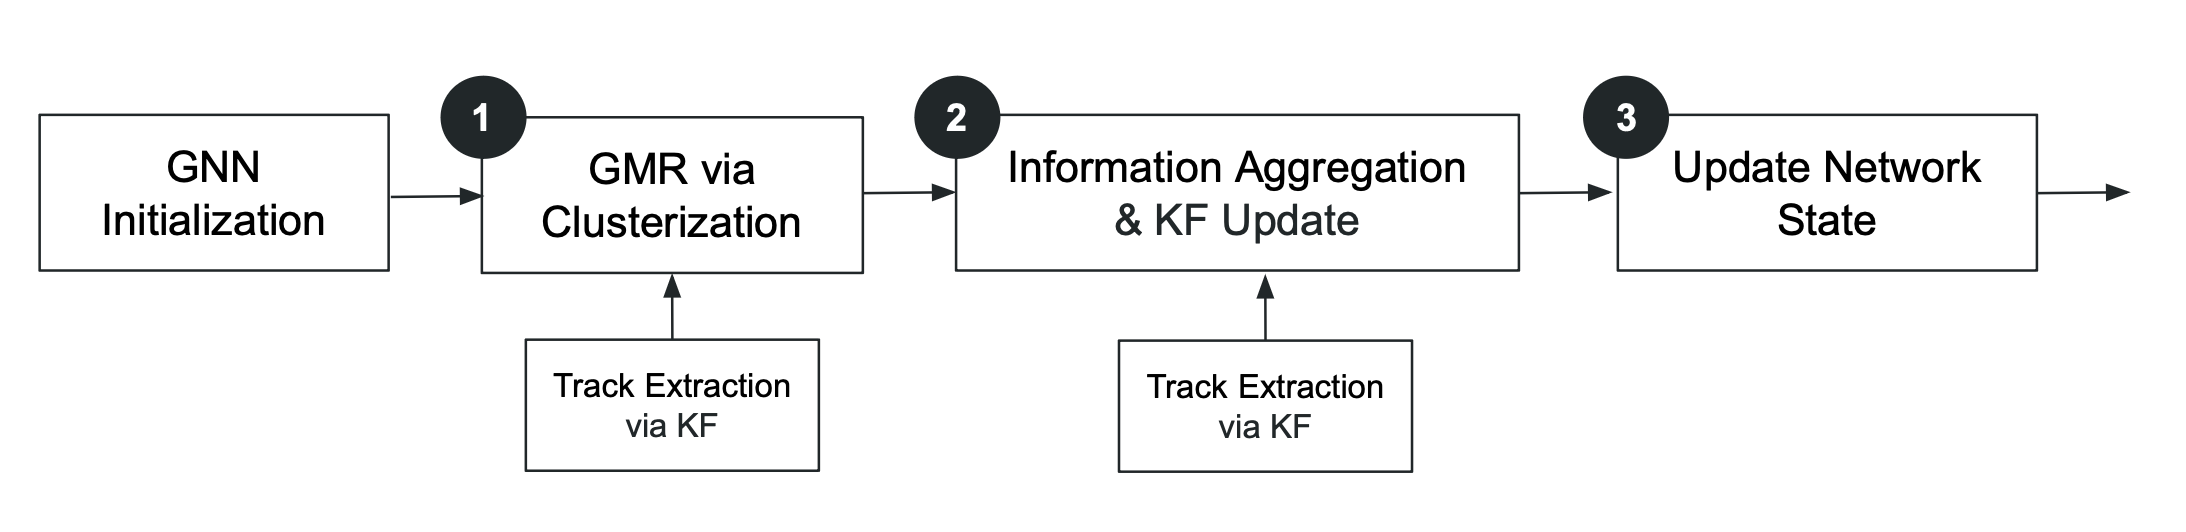
\includegraphics[width=0.98\textwidth]{images/5-gnn-algorithm/gnn-workflow.png}
    \caption{Flow chart illustrating all stages making up an iteration of the GNN-based algorithm. After each stage, a Kalman filter is applied in order to iteratively extract candidates. After stage three, a further Gaussian Mixture Reduction (GMR) stage would be applied repeating the iterations.}
    \label{fig:flowchart}%
\end{figure}




\section{Graph Network Initialization}
\label{gnn-network-initialization}

The graph network is constructed using the Python package \textit{NetworkX} \cite{SciPyProceedings_11}, where track hits are represented as nodes and predicted hit-pairs are represented as edge connections. See Section \ref{chapter-4} for further details on the hit-pair predictor. Following this initial set up, the NetworkX Connected Component Analysis (CCA) is applied \cite{networkx}. CCA is a typical computer vision technique that detects connected regions in data structures and it allows the network to be split into smaller, more manageable graphs referred to as \textit{subgraphs}. Within each subgraph, each node is initialised with a Gaussian vector state representing the local track state estimate, dependent on its neighbourhood. 

An illustration of a node and its neighbourhood is shown in Figures \ref{fig:network-initial-one} and \ref{fig:network-initial-two}, where each pairwise connection forms a track state estimate, $X_{ij}$, initialised with track parameters. See sections \ref{linear-state} and \ref{parabolic-state} for further details on state implementation. All edges are initialised as active, where each edge has an associated prior probability and edge weight. The prior probability $p_{ij}$ of node $i$ and neighbour node $j$ belonging to the same track is determined, assuming a track can produce at most one hit per layer of the detector. The edge weight $w_{ij}$ is a mixture weight for the compatibility of the Gaussian component transmitted from node $i$ to neighbour node $j$, and it represents the strength of the connection. $w_{ij}$ are initialised as uniform dependent on the number of neighbours local to a node and are updated based on how the network evolves. $w_{ij}$ are not to be confused with the traditional weights associated to features within neural networks. All edges in the graph network are bidirectional, such that message passing can occur in both directions with different strength weights. This ensures that the compatibility of the state propagated can be assessed in both directions dependent on its local neighbourhood environment. Given node $i$ and its neighbour nodes $j$, all track state estimates $X_{ij}$, the associated covariances $C_{ij}$, priors $p_{ij}$ and mixture weights $w_{ij}$ are stored at node $i$, forming a weighted Gaussian mixture $g_i(X)$. For any given node $i$, the neighbourhood is approximated by a Gaussian mixture given in Eq. \eqref{eqn:gaussian-mixture}, where $\phi_{ij}$ indicates the Gaussian component of pairwise edge connections between nodes $i$ and $j$.

\begin{equation}
g_i(X) = \sum_{j} w_{ij}\phi_{ij}(X, X_{ij}, C_{ij})
\label{eqn:gaussian-mixture}
\end{equation}


\begin{figure}[htbp]%
    \centering
    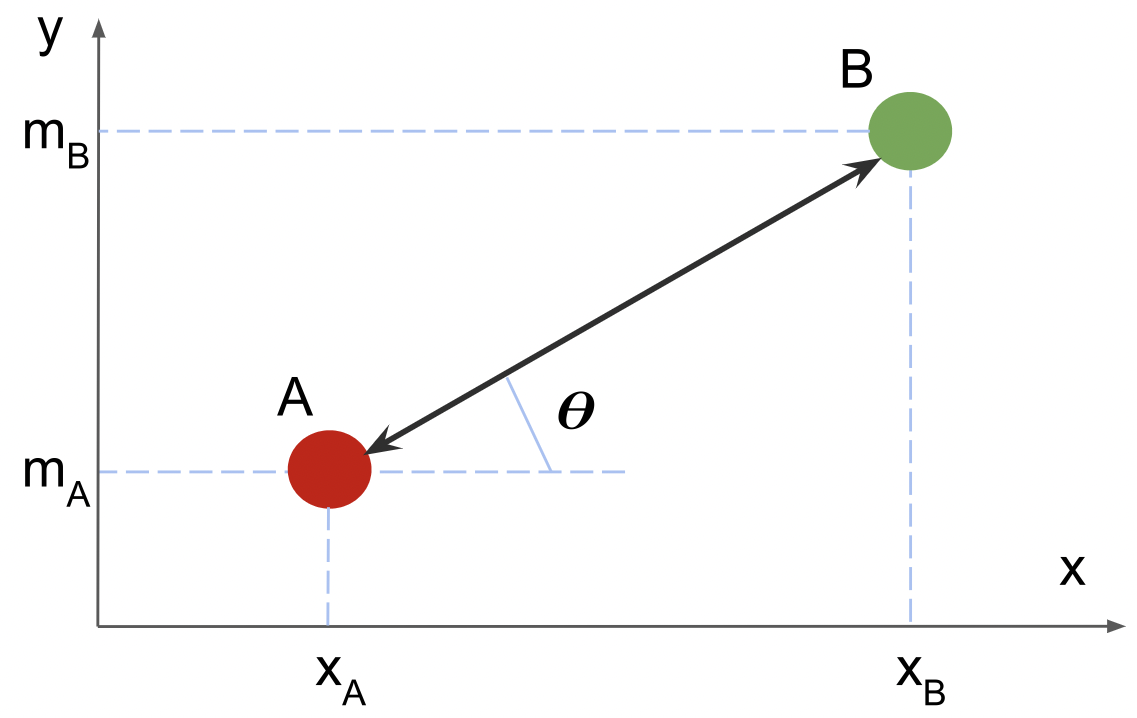
\includegraphics[width=8.7cm]{images/5-gnn-algorithm/network-initialisation-1.png}
    \caption{Illustration showing a bidirectional edge connection between nodes A and B, where $\theta$ is the angle of inclination to node B from the x axis.}%
    \label{fig:network-initial-one}%
\end{figure}

\begin{figure}[htbp]%
    \centering
    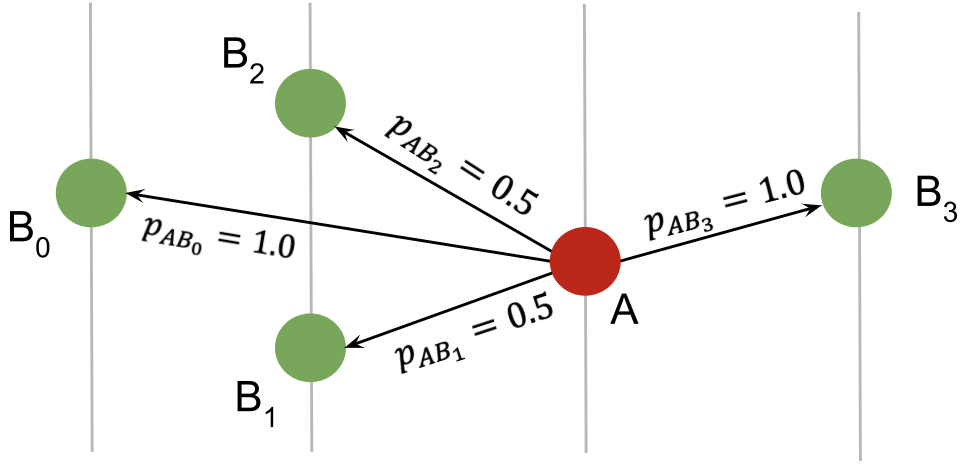
\includegraphics[width=12cm]{images/5-gnn-algorithm/network-initialisation-2.png}%
    \caption{Prior probabilities associated to edge components of the local neighbourhood of node A. Neighbour nodes $B_j$, where each $B_j$ are nodes located on separate detector layers shown by vertical lines. The unidirectional connections show that the state information and prior probabilities are being distributed from node A to its neighbourhood. These entities will differ from nodes $B_j$ distributing to their corresponding neighbourhoods.}%
    \label{fig:network-initial-two}%
\end{figure}




\begin{itemize}
\item Event conversion and graph construction nodes and edges?
\item Track State equations, covariances, derivations, r-z plane and transverse plane
\item edges having priors and weights (strength and compatibility) - because of Gaussian mixture
\item edges act as bidrectional conduits - passing information both ways between nodes
\end{itemize}


\subsection{Linear Track State Model}
\label{linear-state}

\subsection{Parabolic Track State Model}
\label{parabolic-state}


\begin{itemize}
\item In both xy and rz planes, joint track state estimate
\item parabolic model - in local coordinate system of node itself
\item rz joint vector - tau parameter, inverse track inclination
\item how were the covariances dervied and the sigma errors chosen
\end{itemize}

\subsection{Molière Theory of Multiple Scattering}
\begin{itemize}
\item highland formula and handling the error/effects due to multiple scattering for the barrel and endcap in slightly different ways
\end{itemize}
% moliere theory links:
%https://gray.mgh.harvard.edu/attachments/article/337/Techniques%20of%20Proton%20Radiotherapy%20(06)%20Multiple%20Scattering.pdf
%https://pdg.lbl.gov/2005/reviews/passagerpp.pdf





\section{Gaussian Mixture Reduction}
For nodes with a high multiplicity of connections (so called ``hot" nodes), the number of Gaussian components can quickly rise. To make inferences within a reasonable amount of processing time, an intermediate approximation step is used to prevent the number of components of the mixture from exploding. One popular computationally efficient approach for GMR is a clustering-based algorithm. In order to approximate a high order Gaussian mixture by one with lower order, the traditional k-means clustering \cite{kmeans} is used to group together similar track states at each node and hence identify outliers which are then deactivated. As the mixture is reduced, Gaussian components that remain active are merged together to form a single merged state and covariance. This merged state is a higher precision track state estimate at each node and is propagated to further stages.

\begin{itemize}
    \item GMR theory
    \item Clustering, KL divergence
    \item Mahalanobis distance and merging of states
    \item training the optimal threshold using an SVM
    \item feeding in using a fast look-up table
\end{itemize}
\subsection{Learning the Optimal KL Threshold}


\section{Information Aggregation}
\subsection{Message Passing Mechanism}
\subsection{Linear Extrapolation Model}
\subsection{Parabolic Extrapolation Model}
\subsection{Kalman Filter Update}

\begin{itemize}
    \item Information propagation via Message Passing
    \item Extrapolation and Validation
    \item Linear and Parabolic model - 2 different extrapolations for xy componenets of state vector and rz componenet, illustrations here
    \item Kalman Filter Update, OU process for correlated noise
\end{itemize}



\section{Updating Network State}
\label{gnn-updating-network-state}

As the network evolves and certain connections are deactivated, the local track parameter estimates for each node changes. Therefore, the corresponding edge component's $w_{ij}$ are updated. For an edge connection between nodes $i$ and $j$, the updated edge weights $\widetilde{w}_{ij}$ stated in Eq. \eqref{eqn:weights} are computed using the normalised Gaussian measurement likelihood given by Eq. \eqref{eqn:likelihood}. The denominator $\sum_{k}w_{ik}\beta_{ik}$ is the summation of the product of weights and likelihoods in a neighbourhood for a given node $i$. The updated weights $\widetilde{w}_{ij}$ are also divided by the number of detector layers on either side of its neighbourhood $N_S$, in order to account for the probability that a track passing through node $i$ was detected at layer $L$. For a given node, if any $\widetilde{w}_{ij} < 0.1$, these edge connections are automatically deactivated as the likelihood of compatibility of this incoming track state is extremely low. This forms an additional part of the mechanism for edge activation and deactivation. After this update is complete, the iterations repeat and a further GMR would be performed on updated track states. 

\begin{equation}
\beta_{ij} = (2 \pi \lvert S_{ij} \rvert )^{-1/2}  e^{-\Delta \chi^{2}_{ij} / 2}
\label{eqn:likelihood}
\end{equation}

\begin{equation}
\widetilde{w}_{ij} = \frac{1}{N_S} \frac{w_{ij}\beta_{ij} p_i}{\sum_{k}w_{ik}\beta_{ik}}
\label{eqn:weights}
\end{equation}



\section{Track Splitting and Extraction}
\begin{itemize}
    \item CCA
    \item criteria for a good track candidate
    \item Implementation of KFs/ KF track fit
    \item Merging Close Proximity Nodes
    \item Community Detection
\end{itemize}
%Community Detection: divides nodes into various clusters based on edge structure. It learns from edge weights, and distance and graph objects similarly. 

\subsection{Community Detection}

If a subgraph does not meet the criteria to qualify as a good track candidate, a \textit{Community Detection} algorithm \cite{community} is applied in order to further partition the set of nodes. Community Detection is a generalisation of CCA and works by using a distance metric, typically modularity, in order to label nodes as \textit{closely connected}. Modularity is a benefit function that measures the strength of a particular division of a network using the number of edges. A popular modularity maximisation approach is the Louvain method \cite{python_louvain}, which iteratively optimises local communities until global modularity can no longer be improved. An example illustration of a network partition via Community Detection is shown in Figure \ref{fig:community-detection}. Any subgraphs with zero extracted candidates through this procedure are propagated to further stages for additional processing.


\begin{figure}[htbp]
    \centering
    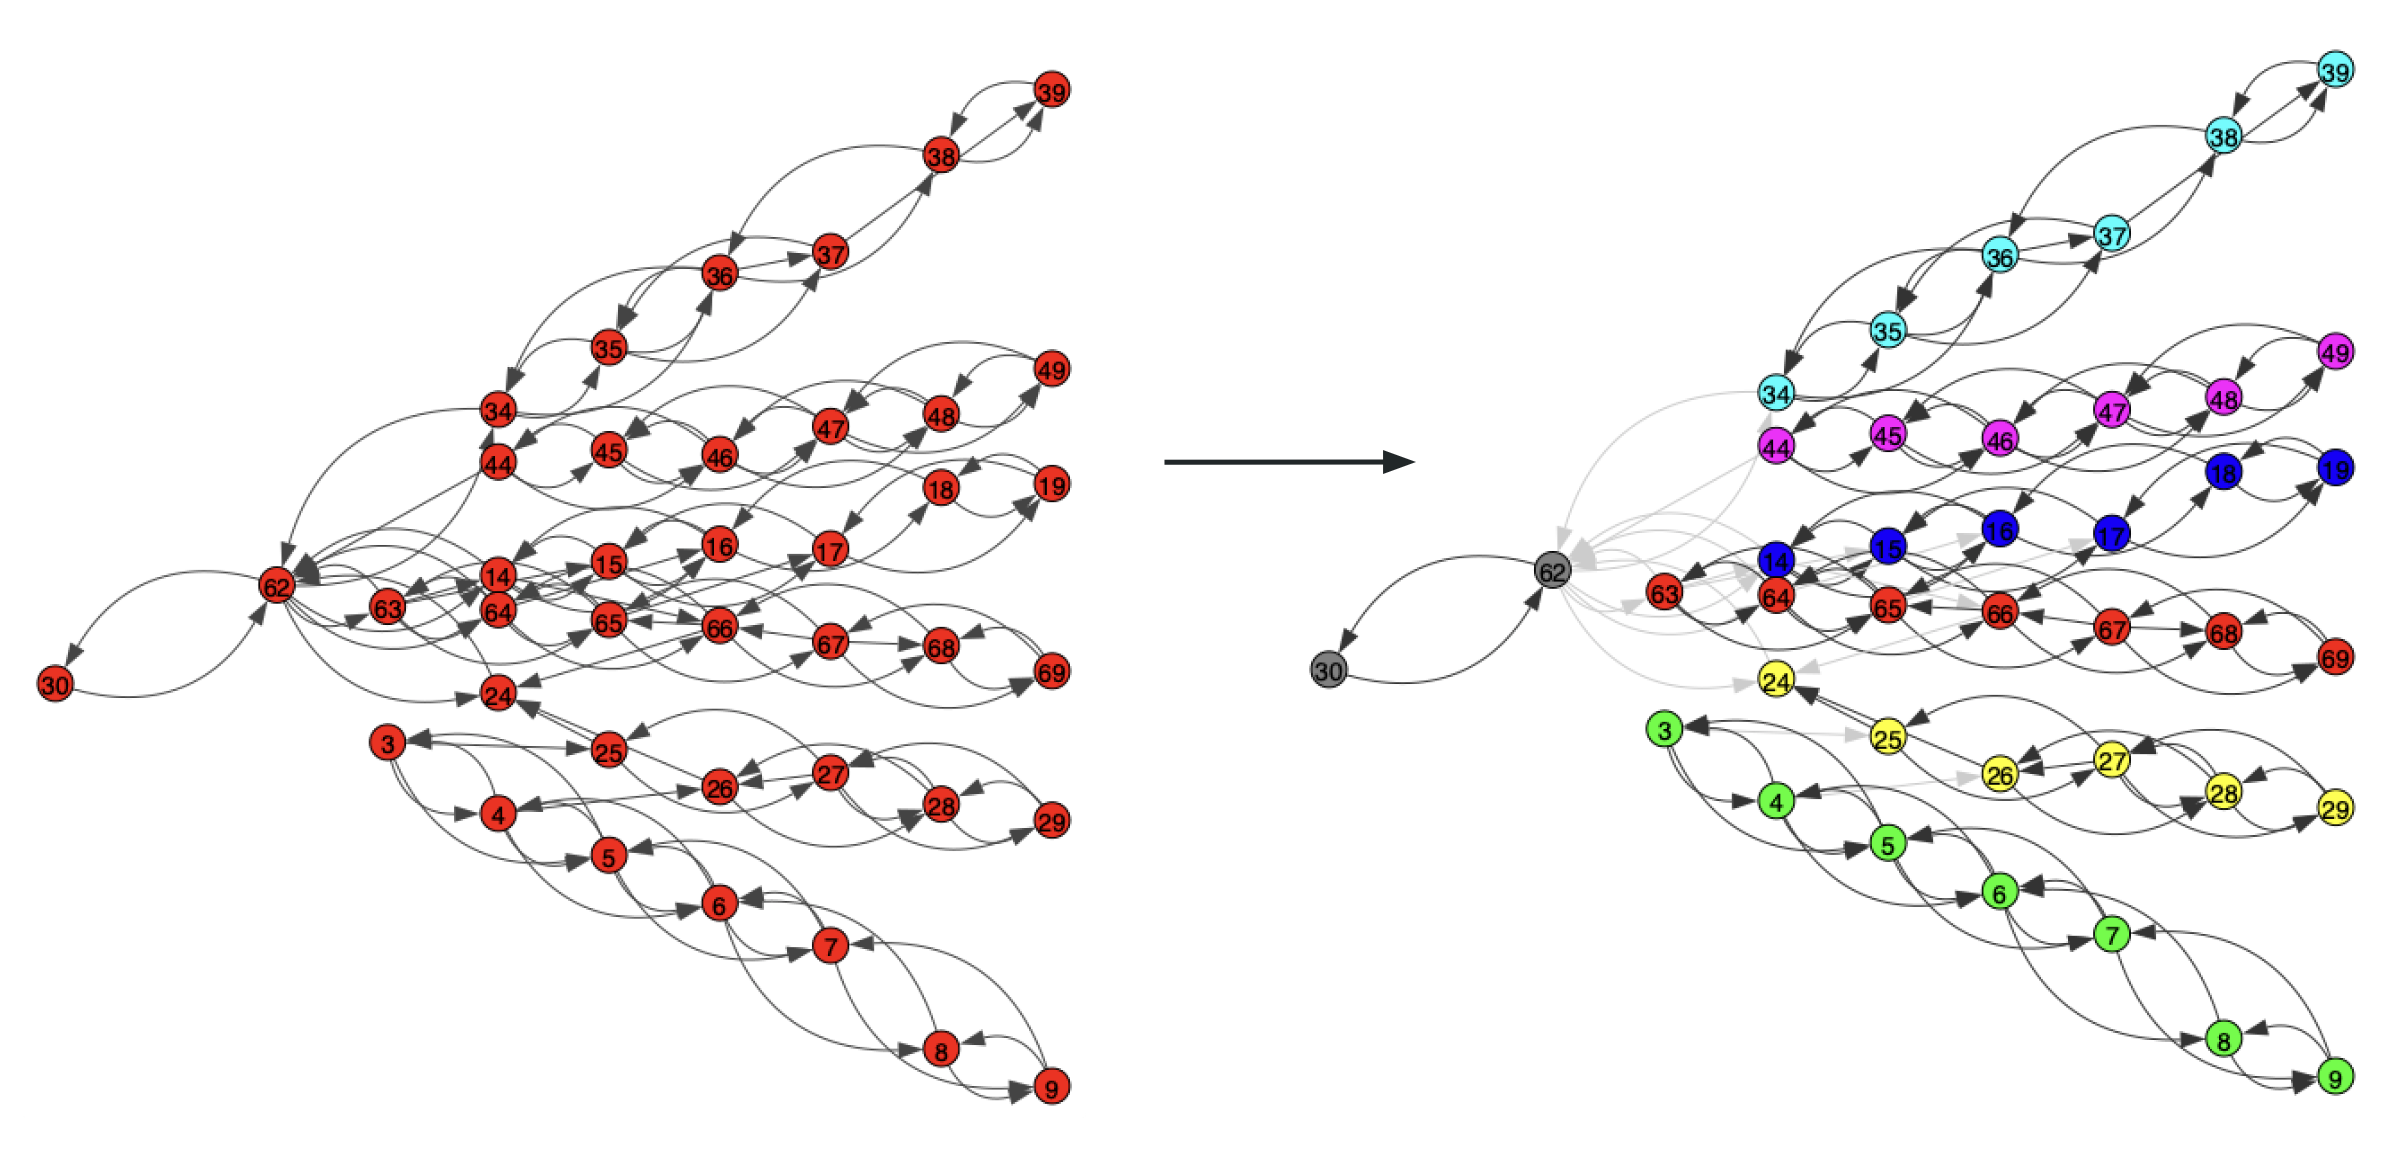
\includegraphics[width=0.98\textwidth]{images/5-gnn-algorithm/community-detection.png}
    \caption{TODO: caption ....}
    \label{fig:community-detection}%
\end{figure}






\section{Implementation of Kalman Filters}
\label{gnn-kf-implementation}

\begin{itemize}
\item emphasis on the use of KFs both in information aggregation stage and in track extraction, both are implemented in different ways, is a useful and unique part to this algorithm
\end{itemize}



\section{Application on a Simple Model}
\label{gnn-application-toy-model}

% TODO: mention here that the linear track state model was used and reference the section

% The excitation and inhibition rules of individual GNN nodes will be designed to facilitate the “simple-to-complex” approach for “hits-to-tracks” association, such that the network starts with relatively “easy” areas of an event (low hit density) and gradually progresses towards more complex areas (high hit density). 

% \begin{itemize}
% \item Application on a simple toy mc model and heat network - track extracted and metrics
% \end{itemize}

A 2-dimensional simulation with seven tracks, each with ten hits, was created, see Figure \ref{fig:ground-truth}. The graph network was formed using a many-to-one mapping of hits-to-nodes, where close proximity hits were merged into one node. The threshold for close proximity hits was determined by considering the distance distribution between hits located in the same layer. In order to build edge connections in the graph network and reduce all possible combinatorics between node pairs, an edge-predictor method was devised. The predictor uses a simple calculation whereby the track inclination of neighbouring nodes is calculated. If the inclination of a neighbour spanning up to two layers apart is within a particular range, then this edge is compatible and a connection is established between the nodes. The network is initialised with its corresponding track state estimates $X_{ij}$, covariance matrices $C_{ij}$ and MC truth particle.

In order to efficiently resolve ambiguities, a method was devised to automatically determine a suitable region for initiating the pattern recognition. For a given node, the variance of edge orientation $\sigma_e^2$ of its neighbourhood was considered. Figure \ref{fig:heat-map} shows a heat map, indicating ``hot'' nodes (white) which represent nodes with a high degree (number of edges associated to the node), whereas ``cold'' nodes (orange - red) indicate regions with fewer ambiguities to resolve. This indicates that the node degree is an indirect characteristic of how complex a local neighbourhood is and provides a method to determine where pattern recognition should begin on a graph network in order to resolve incompatible edge connections. Nodes with $\sigma_e^2 > 0.8$ were temporarily removed and the pattern recognition was initially applied to the remaining network.

\begin{center}
\begin{figure}[htbp]%
    \centering
    \subfloat[\centering Simulation of seven truth tracks]{{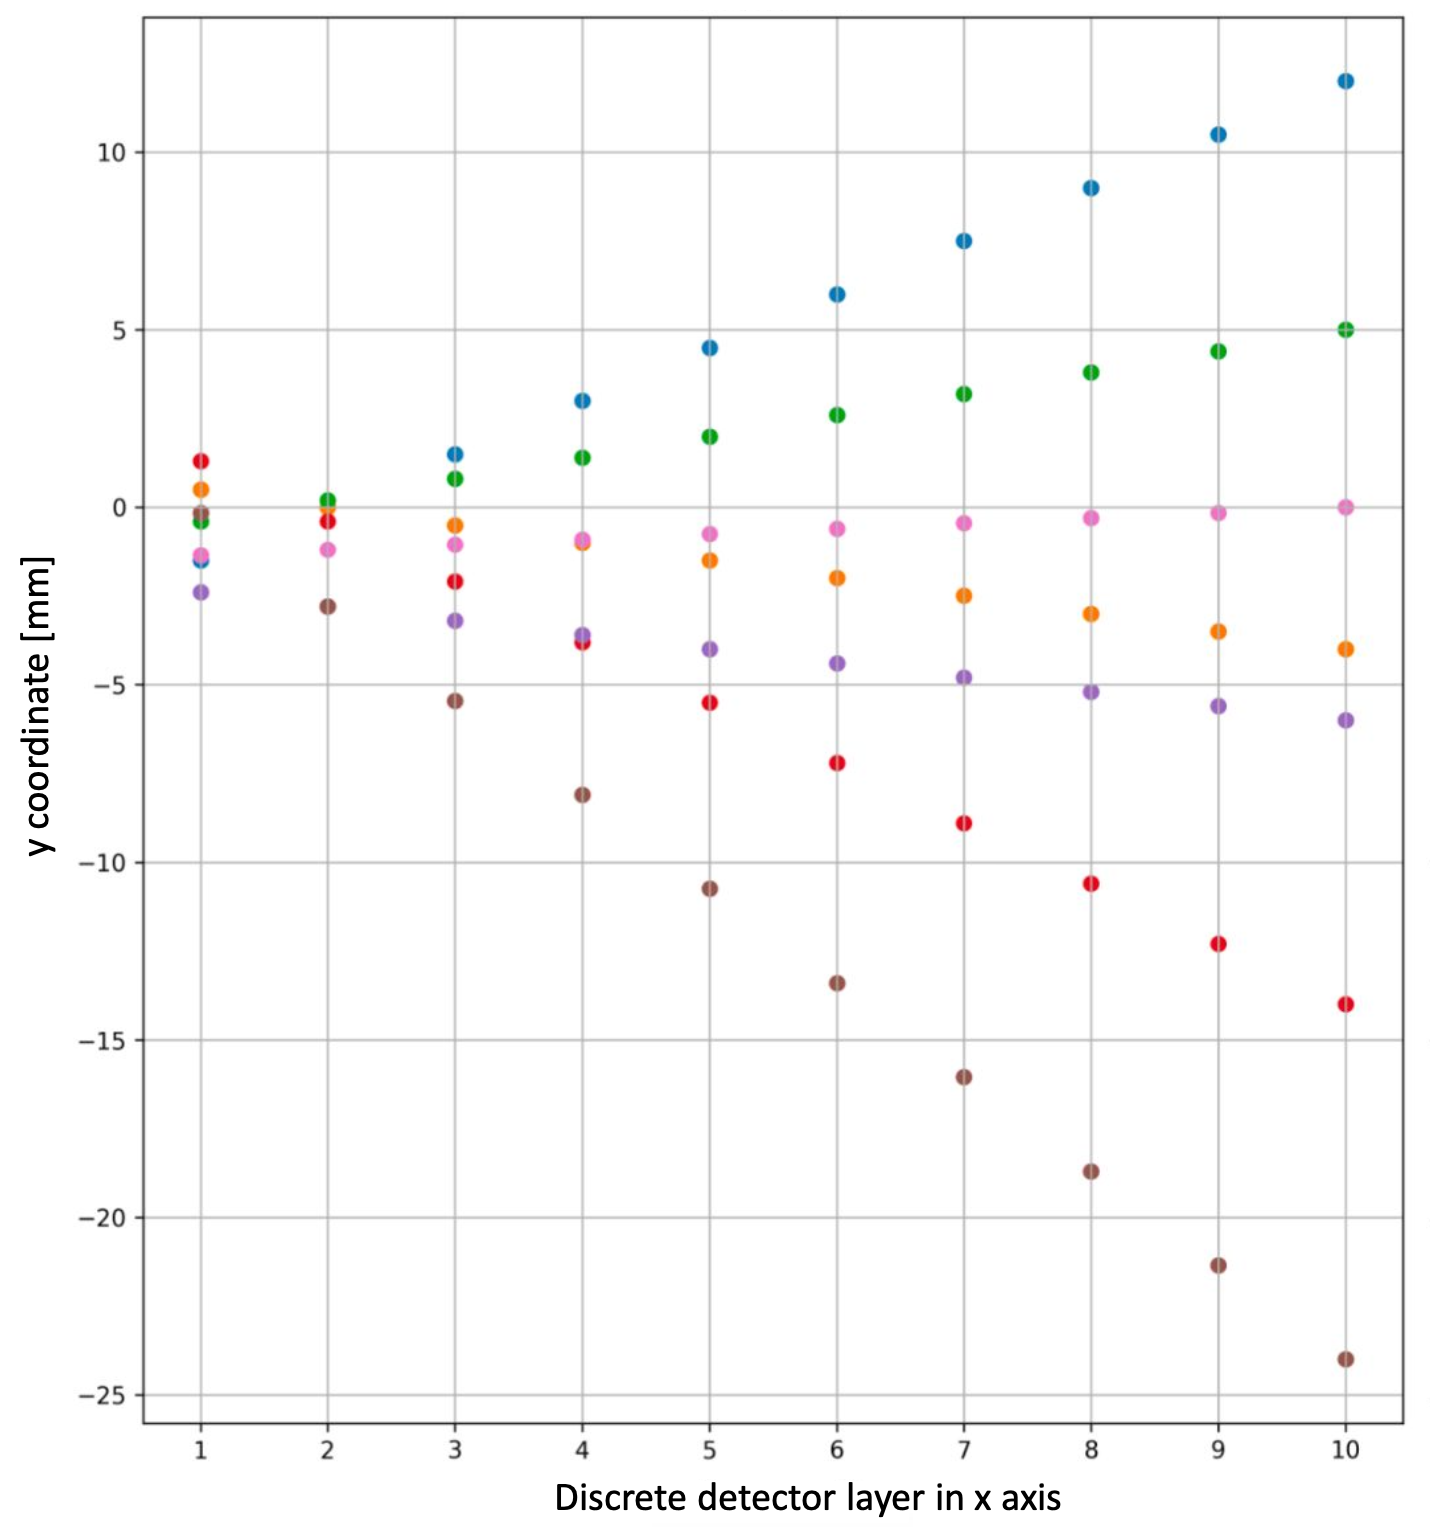
\includegraphics[width=8cm]{images/5-gnn-algorithm/ground-truth.png} } \label{fig:ground-truth}}%
    \hfill
    %\qquad
    \subfloat[\centering Graph network plotted as a node-degree heat map]{{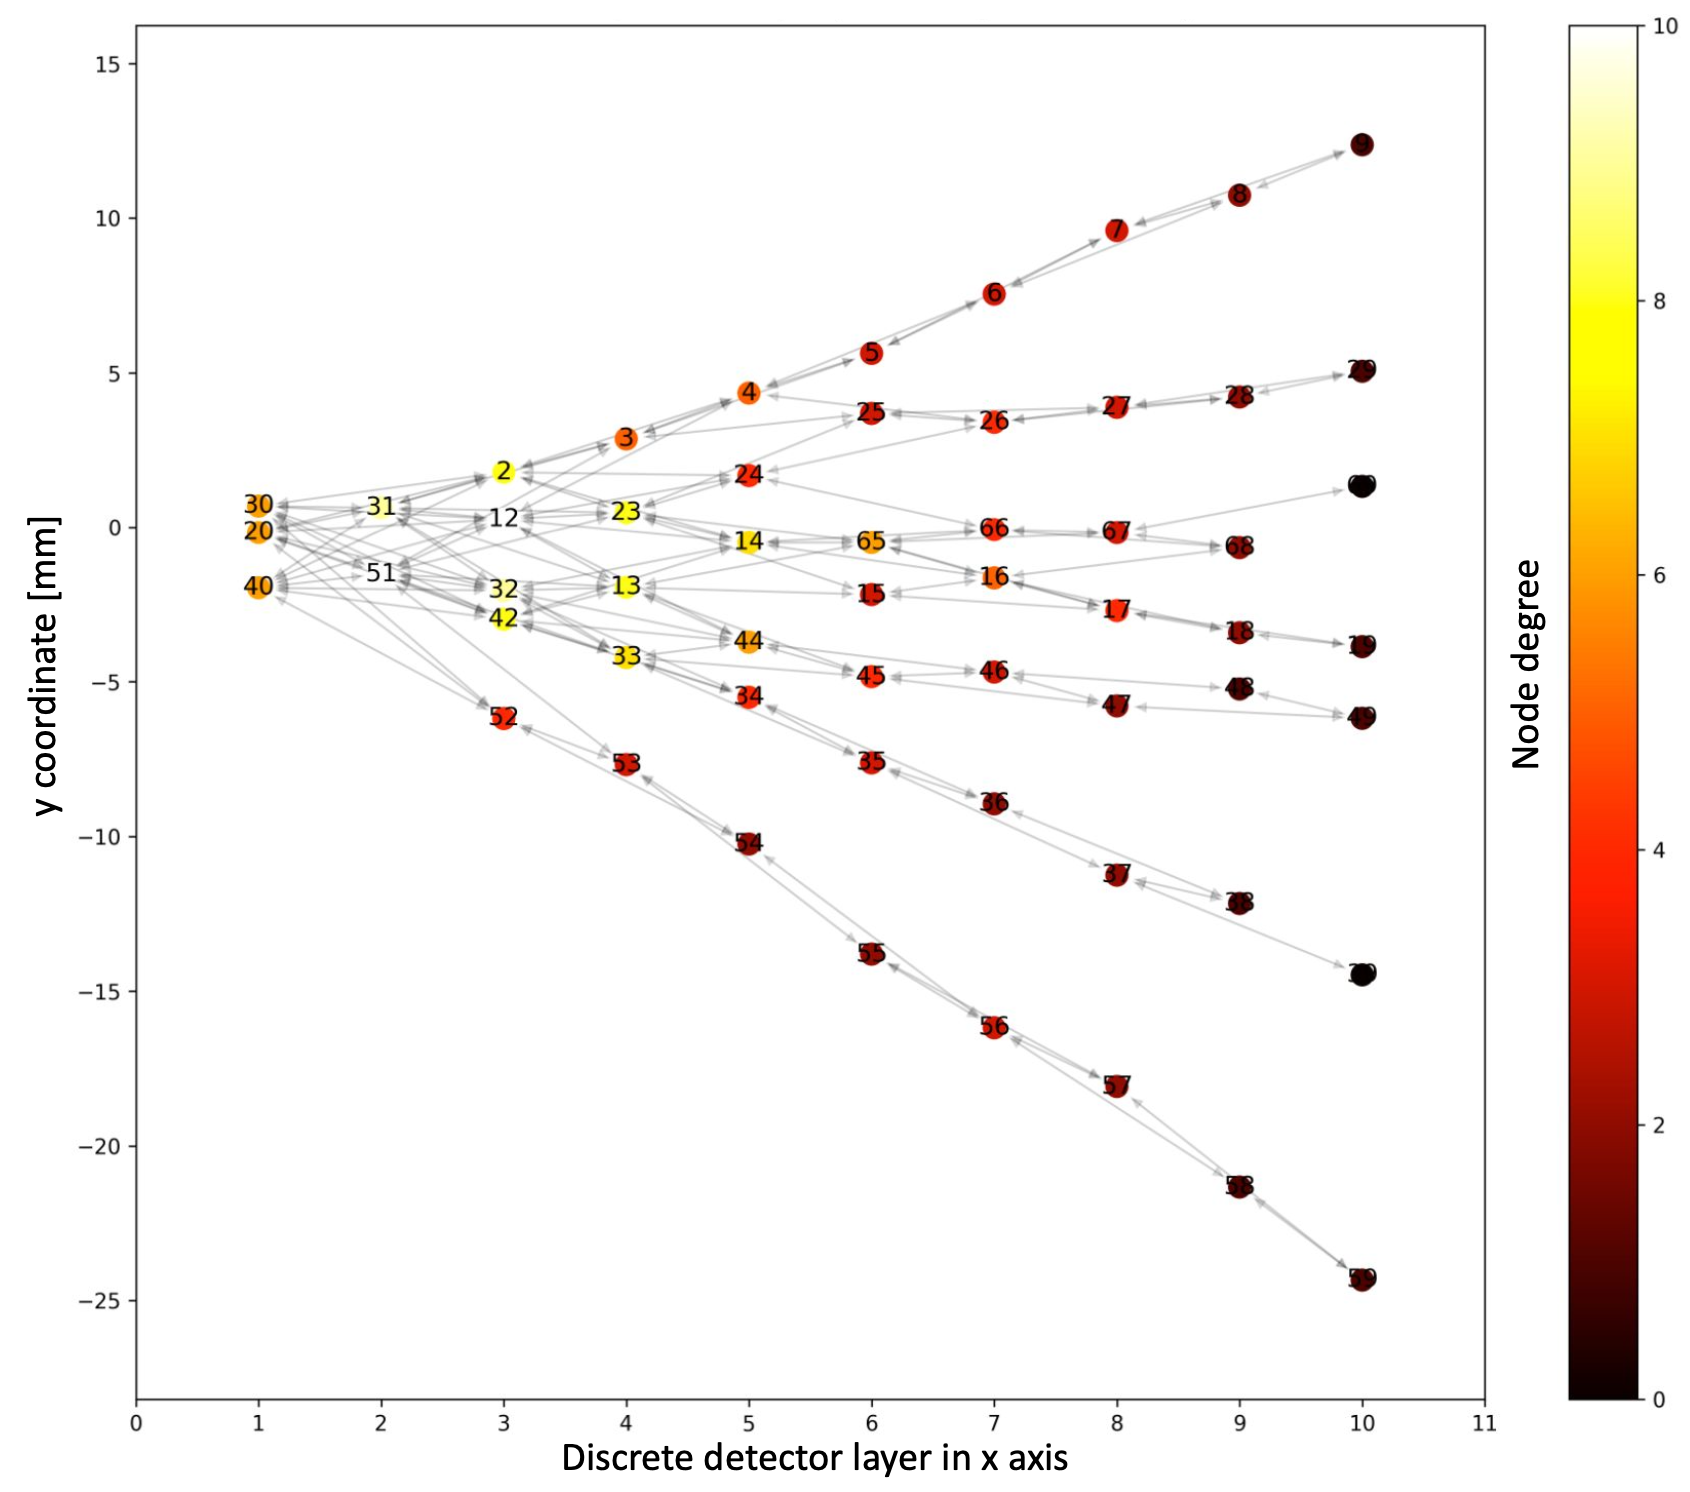
\includegraphics[width=12cm]{images/5-gnn-algorithm/heatmap-network.png} } \label{fig:heat-map}}%
    \caption{a) Simple 2-dimensional simulation of seven truth tracks where each track contains ten hits; one hit per layer. Each colour represents a different track. b)  Conversion of the simulated hits in a), to a graph network containing nodes and edges. Close proximity hits are merged into the same node where necessary and predicted edge connections are formed using a pair predictor. The heat map represents node degree, where ``hot'' nodes (white) contain many edge connections, whereas ``cold'' nodes (orange - red) contain fewer edge connections.}%
    \label{fig:setup}%
\end{figure}
\end{center}




%\section{Conclusions}
